Forward kinematics is the problem of determination of the position and orientation of the end effector given the values for the joint variables. One common way to approach this problem is via utilizing Denavit and Hartenberg (D-H).
In D-H convention each joint is attached with one coordination frame and transformation between these frames are
expressed in four parameters \cite{wikidh}
\begin{itemize}
    \item $d$: offset along previous $z$ to the common normal
    \item $\theta$: angle about previous $z$, from old $x$ to new $x$
    \item $a$: length of the common normal. Assuming a revolute joint, this is the radius about previous $z$
    \item $\alpha$: angle about common normal, from old $z$ axis to new $z$ axis
\end{itemize}
Using the modified version of the DH-parameters results in transformation matrix between axes $n-1$ and $n$ as follows

\begin{equation}
    ^{n - 1}T_n=
    \left[\begin{smallmatrix}
              \cos\theta_n & -\sin\theta_n  & 0 & a_{n-1} \\
              \sin\theta_n \cos\alpha_{n-1} & \cos\theta_n \cos\alpha_{n-1} & -\sin\alpha_{n-1}& -d_n
              \sin\alpha_{n-1} \\
              \sin\theta_n\sin\alpha_{n-1} & \cos\theta_n \sin\alpha_{n-1} & \cos\alpha_{n-1} & d_n
              \cos\alpha_{n-1} \\
              0 & 0 & 0 & 1
    \end{smallmatrix} \right]
\end{equation}
So given all DH-parameters one can find all coordinate frames defined on the robot. These parameters can be presented
on a table, named appropriately as DH-Table, which is commonly provided by the manufacturer. In this case the table
provided by Franka documentary is tabulated in Table \ref{dhtable}. More info can be found on website of Franka Control Interface \cite{frankaweb}.

\begin{table}[ht]
    \caption{DH-parameters}
    \label{dhtable}
    \begin{center}
        \begin{tabular}{|c|c|c|c|c|}
            \hline
            \textbf{\textit{Joint}} & \textbf{\textit{a (m)}} & \textbf{\textit{d (m)}} & \textbf{\textit{ $\alpha$
                (rad)}}& \textbf{\textit{ $\theta$ (rad)}}\\
            \hline
            Joint1 & 0 & 0.333 & 0
            & $\theta_{1}$ \\
            \hline
            Joint2 & 0 & 0 & -$\pi$/2
            & $\theta_{2}$ \\
            \hline
            Joint3 & 0 & 0.316 & $\pi$/2
            & $\theta_{3}$ \\
            \hline
            Joint4 & 0.0825 & 0 & $\pi$/2
            & $\theta_{4}$ \\
            \hline
            Joint5 & -0.0825 & 0.384 & -$\pi$/2
            & $\theta_{5}$ \\
            \hline
            Joint6 & 0 & 0 & $\pi$/2
            & $\theta_{6}$ \\
            \hline
            Joint7 & 0.088 & 0 & $\pi$/2
            & $\theta_{7}$ \\
            \hline
            Flange & 0 & 0.107 & 0 & 0 \\
            \hline
        \end{tabular}
        \label{tab2}
    \end{center}
\end{table}

Utilizing this table one can calculate the end effector pose by multiplying each transformation. This equation as commonly called kinematic chain can be found below in Equation \ref{chain_eq}.

\begin{equation}
    \label{chain_eq}
    T_7^0 = T_1^0 T_2^1 T_3^2 T_4^3 T_5^4 T_6^5 T_7^6
\end{equation}

Figure \ref{robot_img} depicts the provided frames on the robot image.


\begin{figure}[ht]
    \centering
    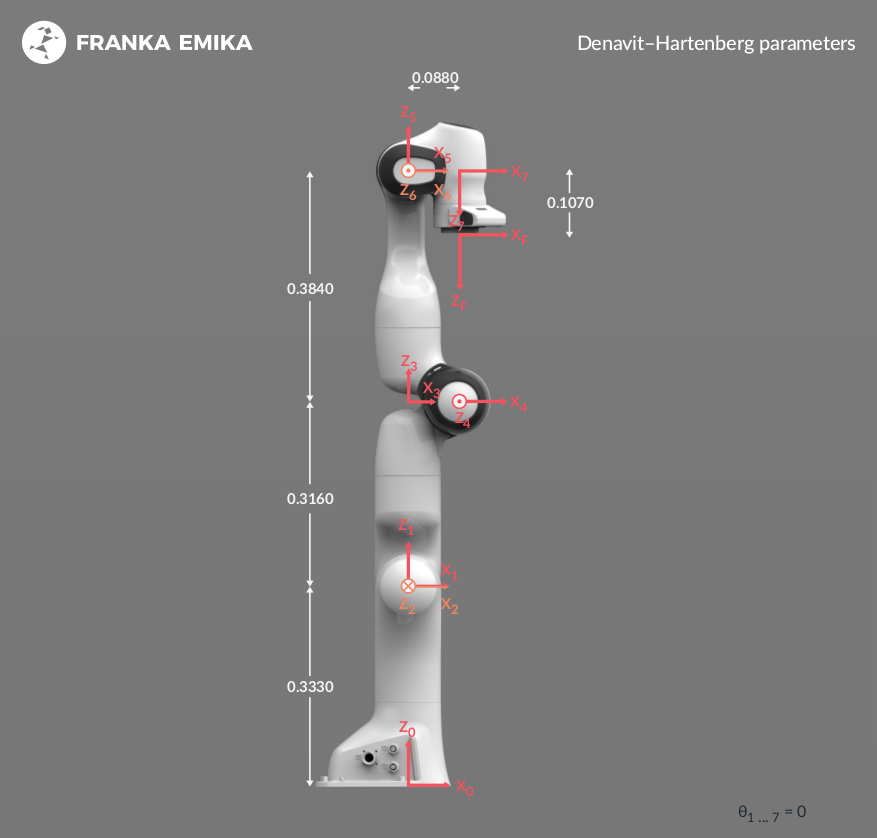
\includegraphics[width=0.45\textwidth]{images/dh-diagram.png}
    \caption{Coordinate frames on the robot}
    \label{robot_img}
\end{figure}
